Although the neutralino is a strong candidate as a DM particle, while the identity of the DM particle remains unknown we will also probe alternative theories. One of these theories is the existence of an extra spatial dimension. This spatial dimension would arise at a high energy scale. The idea is motivated by string theory and M-Theory. Although these will not be discussed at length in this review; an excellent reference for this would be \cite{M-Theory}. 

This has multiple benefits to the standard model, including anomaly cancellation, dynamical electroweak symmetry breaking, prevention of rapid proton decay and, for the importance of this review, a DM candidate \cite{Bertone:2004}. This extra dimension takes several forms. Firstly there is a universal extra dimension (UED) \cite{Appelquist:2000}, in which all paticles in the Standard Model will propagate on. Alternatively, our observable (3+1) dimensional space is a brane existing in a higher (3+$\delta$+1) bulk spacetime \cite{ArkaniHamed:1998rs}. In the Arkani-Hamed, Dimopoulos and Dvali (ADD) model, all Standard Model particles will propagate on 3 spatial dimensions whereas the graviton will propagate in the bulk. There are also intermediate theories, where only certain families will propagate in the bulk, which gives rise to the anomaly cancellations \cite{Dobrescu:2001ae}. For the remainder of this review we shall be focusing on UED. 

UED offers an additional feature not seen in the brane approach. There is remains translational symmetry, leading to a conservation of the momentum in all dimensions. In UED, the extra spatial dimension is flat space compactified onto $S^1$. The method used to reduce the 5-dimensional theory to the 4-dimensional one is known as Kaluza Klein (KK) reduction, which gives a number of interesting properites. We will give a brief, simplified description of this shortly.  To account for chiral fermions, a $Z_2$ symmetry needs to be imposed, i.e. $x^4 \rightarrow - x^4$. Fields can be even or odd under this symmetry.  The compactified space is therefore known as an $S^1/Z_2$ orbifold \cite{Shaw:2014gba}. We will have orbifold fixed points at $x^4 = 0, \pi R$. These fixed points will break translational symmetry in the $x^5$ direction, also breaking momentum conservation. A symmetry known as the KK number, coming from momentum conservation, is therefore also broken by this $Z_2$ symmetry. But a residual conservation is seen; the KK-parity is given by $(-1)^m$. All modes with odd $m$ will be charged under this parity. It is also clear there will be mixing between KK modes due to this broken momentum conservation. The DM candidate emerging from these modes is known as the lightest Kaluza-Klein particle (LKP), where $m=1$ \cite{Servant:2002}. It was first discussed by Kolb and Slansky, who coined it the pyrgons \cite{Kolb:1983fm}. The LKP is stable as it is protected by KK-parity, at tree-level. As stated, a DM candidate must be stable, electrically neutral and non-baryonic. The best candidates from this theory then become the first level KK modes of the neutral gauge bosons (the photon and Z boson) and the neutrino. Following the notation of \cite{Servant:2002}, we will refer to the first photon mode as $B^{(1)}$. 

Returning to the KK modes, first consider imposing periodic boundary conditions on our orbifold (we consider fields even under $Z_2$), expanding in Fourier modes gives us particles in the form (suppressing spacetime indices),
\begin{equation}
    \psi(x^\mu, x^4) = \sum_{n\in \mathbf{Z}} e^{(i n x^{4} / R)} \phi_n(x^\mu)
\end{equation}
where the quantisation of the momentum in the extra dimension, $x^4$, keeps the wavefunction single-valued \cite{Tong:2009np}. Here $R$ is the radius of the orbifold. For completeness, $\phi_n^* = \phi_{-n}$. Using the equation of motion, it can be seen that there are mass modes of $M_n^2 \sim n^2 / R^2$, and we have found the tower of KK modes. The zero modes here correspond to Standard Model states \cite{Shaw:2014gba}. A detection of the higher modes, as seen by CERN, would appear as periodic spikes in the number of events as a function of centre of mass energy. So far no such signal has been found.

The relic density of $B^{(1)}$ has been computed in \cite{Servant:2002}, where they considered coannihilations with the next lightest KK particle, $e^{(1)}_R$, the right handed first KK mode of the electron. It can been seen in Figure \ref{fig:RelicDensity}. It was assumed all other modes are too heavy to contribute. The relative mass difference between the LKP and the NLKP was inputted as 
\begin{equation}
    \Delta = \frac{m_{NLKP} - m_{LKP}}{m_{LKP}}
\end{equation}
It is important to note that the density of the $B^{(1)}$ is increased when considering $e^{(1)}_R$ than without. This is because the cross section for self-annihilation is larger than the cross-section for coannihilation; the particles will decouple at a similar time with coannihilation as without, and the remaining $e^{(1)}_R$ will decay into $B^{(1)}$. The green region is the required relic density, which corresponds to masses between $0.6 - 1.2$ TeV depending on the model considered.
\begin{figure}[htbp]
    \centering
    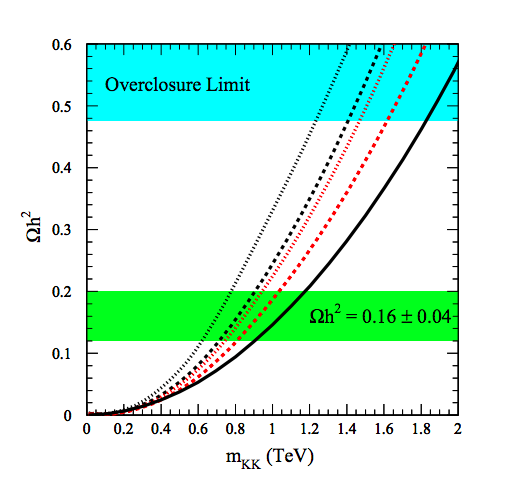
\includegraphics[width=0.6\textwidth]{RelicDensity.png}
    \caption{\label{fig:RelicDensity}The relic density of $B^{(1)}$ against its mass. The solid line considers $B^{(1)}$ alone, and the dashed and dotted lines correspond to the case in which there are one or three flavors of nearly degenerate $e^{(1)}$ respectively. For each case, the black curves denote the case $\Delta$ = 0.01 and the red curves $\Delta$ = 0.05. Figure taken from \cite{Servant:2002}.}
\end{figure}

The first mode of the neutrino, $\nu^{(1)}$ has also been considered as a possible candidate. It satisfies stable, electrically neutral and non-baryonic conditions required from WIMPs. Its relic density has been discussed in further detail in \cite{Servant:2002}.

There are other nuances to consider with these particles, these have been discussed in other papers at length. We have used mostly tree-level consideration, but for a paper on the radiative correction to the mass of the KK particles, see \cite{Cheng:2002iz}. They consider the fact that the extra dimensions in our theory will violate Lorentz symmetry, giving corrections to the mass beyond tree-level. We would also stumble upon log divergences and interactions between only even or odd KK modes. Further discussion on direct detection can be found in \cite{Servant:2002hb}. Recent experimental bounds on $R$ are given by $R \lesssim 40 ~\rm \mu m$ \cite{Kapner:2006si}.